%!TEX  root = main.tex
\chapter{Prototypage et validation du \emph{framework ExecuteEA}}
\label{ch:implem}

\PartialToc


\section{Environnement retenu : la plate-forme Eclipse}

Notre choix s'est orienté vers la plate-forme Eclipse et ce pour plusieurs
raisons.

Tout d'abord, il s'agit d'une plate-forme open-source dont l'utilisation est
particulièrement répandue dans la communauté IDM. En effet, la plate-forme
Eclipse abrite le projet
\gls{emf}\footnote{http://www.eclipse.org/modeling/emf/} qui a pour objectif de
doter Eclipse d'outils orientés IDM.

Ensuite, \gls{emf} s'appuit sur les standards du domaine. Par exemple, le méta-
métamodèle Ecore, pilier central de \gls{emf}, se base sur le standard
\gls{mof}\footnote{http://www.omg.org/mof/} . Aure exemple, le langage de
contraintes OCLinEcore se base sur le standard \gls{ocl}. OCL et MOF sont des
standard de l'OMG.

Puis, \gls{emf} se décompose en sous-projets orientés vers différents aspects de
l'IDM tels que la méta-modélisation, la transformation de modèle, les éditeurs
graphiques de modèles, les langages spécifiques au domaine. \gls{emf} offre
ainsi un environnement personnalisable pour mettre en œuvre une approche IDM.

Enfin, il s'agit de la plate-forme retenu par le projet Pomme du département
MIRE, dans lequel s'inscrit nos travaux de thèse. Le projet Pomme vise à
réaliser un outil pour la co-simulation des trois domaines qui compose un Smart
Grid~: SI, infrastructure électrique, infrastructure de télécommunication.

Pour ces travaux de thèse, nous avons donc retenu~:

\begin{itemize}

    \item Ecore pour la méta-modélisation~;

    \item OCLinEcore pour l'expression de contraintes et de requêtes sur le métamodèle~;

    \item Le langage Acceleo pour les transformations de modèle~;

    \item Le plugin Papyrus\footnote{https://eclipse.org/papyrus/} pour la simulation
    des modèles d'architecture. Papyrus est compatible avec le standard fUML et
    permet donc d'exécuter les diagrammes de classes et d'activité. 

\end{itemize}


\section{Réalisation et difficultés rencontrées}

    \subsection{Implémentation du métamodèle EA2M avec Eclipse Modeling Framework}

    Le métamodèle EA2M est le pilier central du \emph{framework ExecuteEA}. Nous
    l'avons implémenté à l'aide de \gls{emf}. Il est donc conforme au méta-
    métamodèle Ecore. EMF génère automatiquement un éditeur de modèle à partir
    d'un métamodèle conforme à Ecore. Cet éditeur permet de créer des modèles
    d'architecture d'entreprise conformes au métamodèle EA2M ainsi implémenté.
    La figure~\ref{fig:editeur_modele1} et la figure~\ref{fig:editeur_modele2}
    sont une capture d'écran de l'éditeur de modèles générée automatiquement à
    partir du métamodèle EA2M. L'utilisateur a le choix de créer une vue métier,
    fonctionnelle, applicative ou intégration et pour chacune des vues il peut
    choisir de créer un aspect objectif, processus ou information.


    \begin{figure}[!htbp]
     \begin{center}
      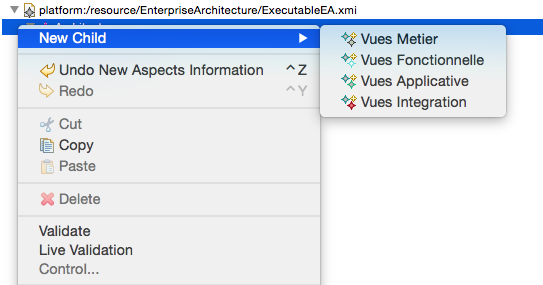
\includegraphics[width=0.8\textwidth]{figures/5_implementation/editeur_modele1.png}
     \end{center}
     \caption{Edition de modèles d'architecture d'entreprise avec ExecuteEA\\création de vues}
     \label{fig:editeur_modele1}
    \end{figure}

    \begin{figure}[!htbp]
     \begin{center}
      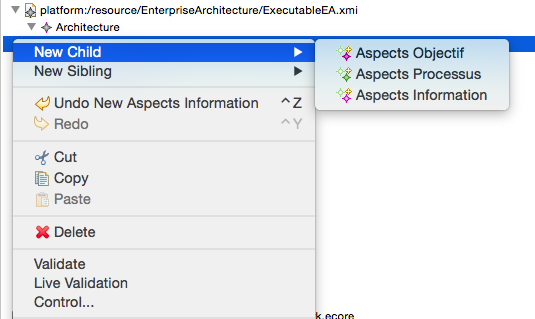
\includegraphics[width=0.8\textwidth]{figures/5_implementation/editeur_modele2.png}
     \end{center}
     \caption{Edition de modèles d'architecture d'entreprise avec ExecuteEA\\création d'aspects}
     \label{fig:editeur_modele2}
    \end{figure}

    La figure~\ref{fig:modeleEA} représente une capture d'écran d'un modèle d'architecture
    d'entreprise créé avec l'éditeur de modèle ExecuteEA.

    \begin{figure}[!htbp]
     \begin{center}
      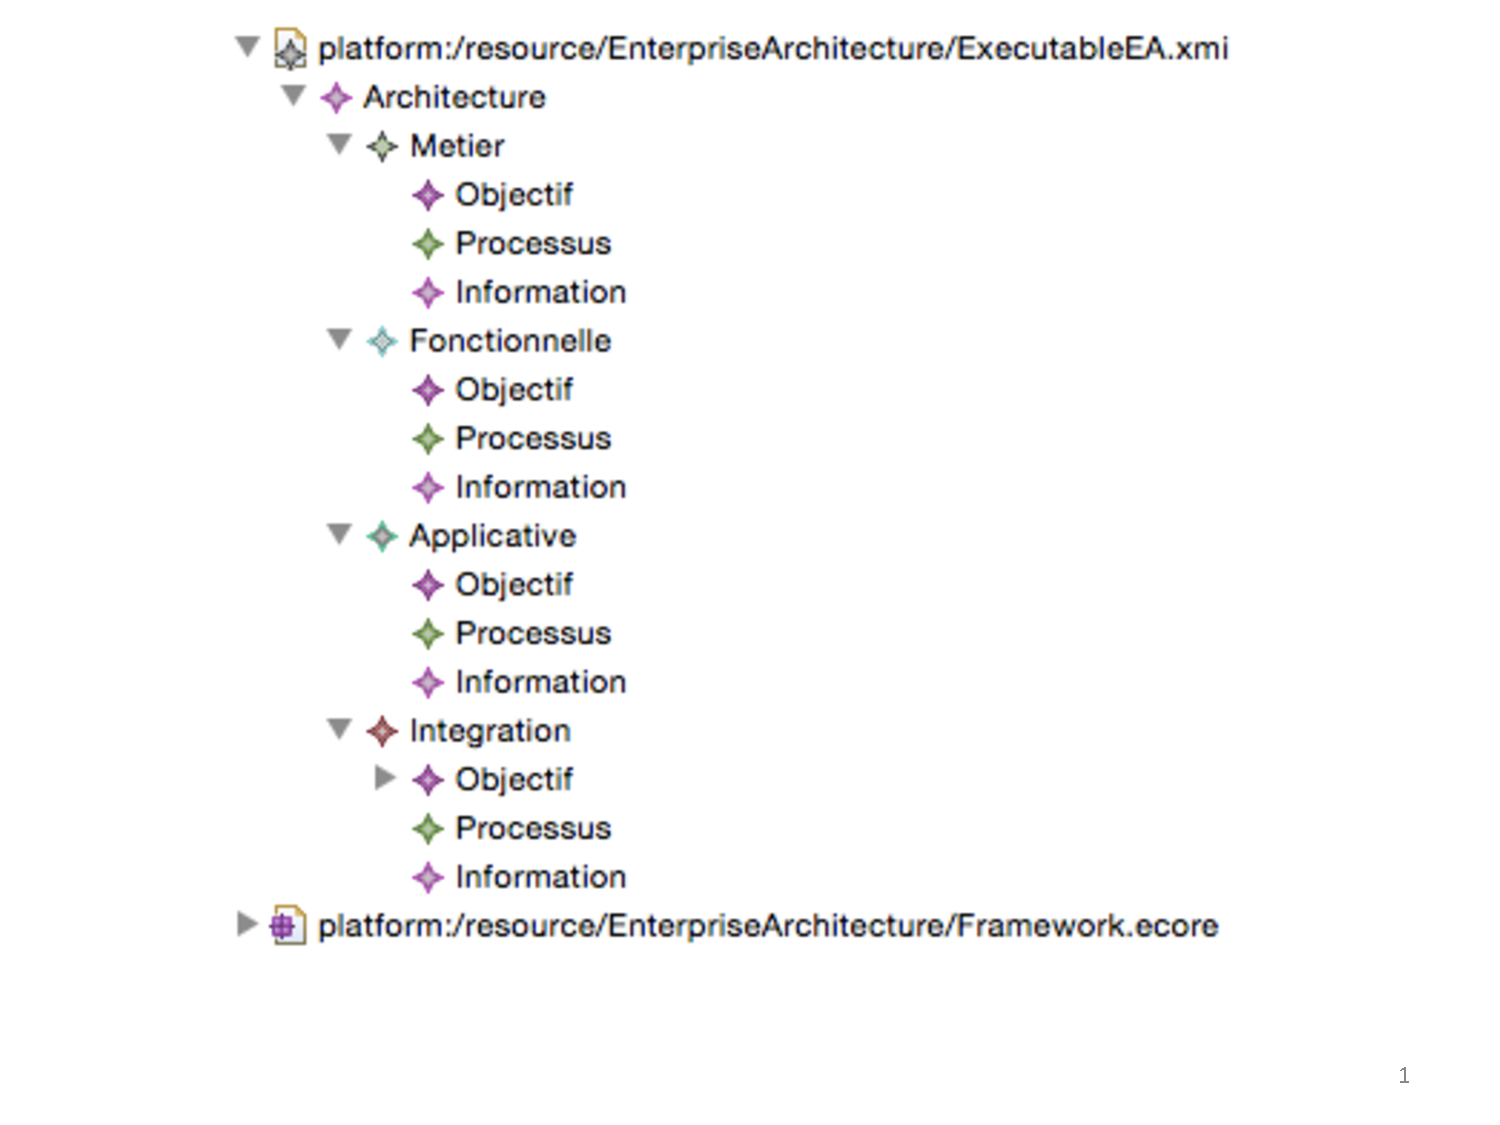
\includegraphics[trim=0cm 3cm 0cm 0cm, width=0.8\textwidth]{figures/5_implementation/modele_ea.pdf}
     \end{center}
     \caption{Modèle d'architecture d'entreprise créé avec l'éditeur ExecuteEA}
     \label{fig:modeleEA}
    \end{figure}

    La difficulté majeure rencontrée en implémentant le métamodèle EA2M a été de
    trouver le bon équilibre entre deux impératifs~: (1) implémenter le
    métamodèle en utilisant des concepts et des relations qui font sens d'un
    point de vue EA, en se gardant la possibilité de l'étendre facilement,
    notamment, par d'autres aspects ou d'autres vues, (2) tout en créant un
    éditeur suffisamment contraignant pour créer des modèles d'architecture
    corrects. Par exemple, utiliser uniquement le mécanisme de multiplicités
    entre la classe abstraite \q{Vue} et la classe \q{Architecture} ne contraint
    pas le modélisateur à ne pas créer plusieurs fois le même type de vue pour
    une seule architecture. Un modèle avec deux vues métier serait par
    conséquent conforme au métamodèle mais ne serait pas pertinent d'un point de
    vue EA.

    Nous avons donc exprimé des contraintes avec OCLinEcore pour ne créer que
    des modèles pertinents tout en gardant un métamodèle pertinent d'un point de
    vue purement EA.  Une contrainte est une expression à valeur booléenne qui
    sert à préciser ou restreindre n'importe quel élément du métamodèle.

    La figure~\ref{fig:contraintes_ocl_architecture} illustre le métamodèle
    EA2M, implémenté à l'aide d'\gls{emf}, sous une forme textuelle\footnote{EMF
    est doté d'une éditeur graphique qui permet de créer des métamodèles de
    manière graphique (par \emph{drag and drop}) sous la forme d'un diagramme de
    classe et de générer le même métamodèle sous une forme textuelle.}. Il
    s'agit donc de la classe \q{Architecture} à la quelle on a ajouté des
    contraintes de type \q{invariant} pour qu'elle ne contiennent pas de vue du
    même type.

    \begin{figure}[!htbp]
     \begin{center}
      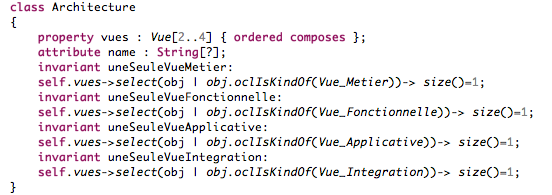
\includegraphics[width=0.8\textwidth]{figures/5_implementation/ocl_in_ecore_vue.png}
     \end{center}
     \caption{Contraintes OCLinEcore attachées à la classe \protect\q{Architecture} }
     \label{fig:contraintes_ocl_architecture}
    \end{figure}

    \subsection{Exécution des modèles d’architecture avec Papyrus}
    \label{sec:opaque_action_papyrus}

    Papyrus est un atelier de modélisation orienté IDM doté d'un moteur
    d'exécution de diagrammes fUML conformément aux spécifications de l'OMG.
    Nous l'avons utilisé pour simuler l'architecture. Comme présenté dans le
    chapitre~\ref{ch:proposition}, nous proposons de simuler l'ensemble de
    l'architecture en la pilotant par les modèles.  La difficulté majeure
    rencontrée à cette étape de l'implémentation a été de réussir à exécuter des
    comportements difficile à modéliser avec un diagramme
    UML\footnote{Typiquement, l'optimisation d'une affectation de véhicules
    électriques à des tournées d'agents qui intervient dans le cas d'études
    présenté dans la suite de ce chapitre}. Le principe de simulation pilotée
    par les processus métier, tel que présenté dans la
    figure~\ref{fig:Simulation_Approche}
    (page~\pageref{fig:Simulation_Approche}), exige de plus de faire appel aux
    modules de la vue applicative.
    
    Le standard fUML a prévu l'exécution de comportements spécifiques difficiles
    à modéliser avec  des diagrammes d'activité. Il dédie à cet effet une
    action\footnote{Dans les spécifications d'UML et de fUML, une action est une étape
    unitaire à l'intérieur d'une activité. Une activité est donc composée de
    plusieurs actions.} spécialisée~: l'\emph{OpaqueAction}. Papyrus s'appuie
    sur le moteur d'exécution Moka pour simuler les diagramme fUML. Moka est
    conforme à la sémantique d'exécution spécifiée par l'OMG pour fUML. Or la
    sémantique d'exécution de l'\emph{OpaqueAction} n'a pas encore été
    spécifiée. Le standard fUML est en effet relativement récent\footnote{La
    première version de fUML a été publiée par l'OMG en févier 2011} et n'a pas
    encore été entièrement spécifié. Pour cette raison, le moteur d'exécution
    Moka ne prend pas en charge l'exécution de l'\emph{OpaqueAction}

    Cependant, Papyrus donne la possibilité d'étendre le moteur d'exécution Moka
    et en attribuant le comportement souhaité à \emph{OpaqueAction} et en
    l'exécutant comme les autres actions au cours d'une simulation de diagramme
    d'activité. Cette extension n'a toutefois pas été facile à implémenter. Les
    tutoriels mis à disposition par l'équipe de développement du module Moka
    sont utiles pour une utilisation basique mais ne répondent à des besoins
    d'utilisation pointues telle que l'extension du moteur d'exécution
    disponible. À cet effet, nous avons sollicité l'aide de contributeurs au
    développement du module Moka et nous nous sommes également appuyé sur un
    stagiaire en dernière école d'ingénieur. Le comportement de
    l'\emph{OpaqueAction} mis en œuvre dans ces travaux de thèse consiste donc à
    appeler un module extérieur durant l'exécution d'un diagramme d'activité
    fUML et à retourner le résultat fourni par le module à l'action ou
    l'activité suivante.

    Dans la suite de ce chapitre, nous éprouvant le \emph{framework ExecuteEA}
    ainsi doté d'un environnement de modélisation et de simulation de modèles
    d'architecture. La validation est faite à travers le cas d'étude de la
    gestion d'une flotte de véhicules électrique. Nous avons créé à cet effet
    (1) les modèles d'architecture d'entreprise requis par les différentes vues
    et selon les aspects spécifié par \emph{ExecuteEA} en adoptant les langages
    prescrit par le \emph{framework}, et (2) les transformations de modèle
    nécessaires. Nous avons ensuite analyser l'architecture obtenue.


\section{Concrétisation de l'approche avec un cas d'étude}

    Les contraintes de temps et de confidentialité ne nous ont pas permis
    d'éprouvé le framework ExecuteEA sur une architecture d'entreprise à taille
    réelle. Pour cette raison, le cas d'étude concerne plutôt un seul processus
    métier faisant intervenir plusieurs tâches et sa déclinaison sur les vues
    fonctionnelle et applicative. Il s'agit de la gestion d'une flotte de
    véhicules électriques. Ce cas métier nous permet néanmoins de concrétiser
    les propositions de ces travaux de thèse et de parer à la difficulté
    d'évaluer quantitativement ces propositions.

    \subsection{Présentation du cas d'étude~:\\la gestion d'une flotte de véhicules électriques}

    Les raisons motivant le choix de ce cas d'étude pour éprouver le framework
    proposé dans ces travaux de thèse ont été discutées dans le
    section~\ref{motivations_cas_metier} (voir
    page~\pageref{motivations_cas_metier}).  Dans cette partie, nous nous
    contentons donc simplement de le présenter.

    Il s'agit du processus d'affectation de véhicules à des tournées d'agents
    (par exemple, une tournée d'un agent EDF qui relève les compteurs chez les
    client, ou encore qui fait des réparations le réseau électrique).  La
    mobilité électrique implique un changement de paradigme pour le gestionnaire
    de flotte de l'entreprise. D'une part, le véhicule électrique est limité par
    son autonomie et ne peut donc pas effectuer n'importe quelle tournée.
    D'autre part, la recharge d'un véhicule électrique implique des contraintes
    (temps de recharge, disponibilité des bornes) que ne présente pas le
    véhicule thermique qui se contente d'un plein de carburant.
    
    Dès lors, le processus d'affectation de véhicules aux tournées des agents,
    la gestion de la flotte de véhicules dans son ensemble et donc le SI qui
    l'implante sont fortement impactés par l'arrivée massive des véhicules
    électriques. Nous proposons de modéliser de cas d'étude selon en mettant en
    œuvre le \emph{framework ExecuteEA}. Nous adoptons donc l'approche
    conceptuelle préconisée par le framework (voir
    figure~\ref{fig:approche_conceptuelle},
    \pageref{fig:approche_conceptuelle}). Nous commençons donc par modéliser des
    différentes vues d'architecture —~métier, fonctionnelle, applicative et
    intégration~— en respectant le cadre structurant du \emph{framework
    ExecuteEA} (illustré par la figure~\ref{fig:cadre_structurant},
    page~\pageref{fig:cadre_structurant}) ce qui nous permettra ensuite
    d'analyser la structure et le comportement de l'architecture ainsi obtenue.

    \begin{figure}[!htbp]
     \begin{center}
      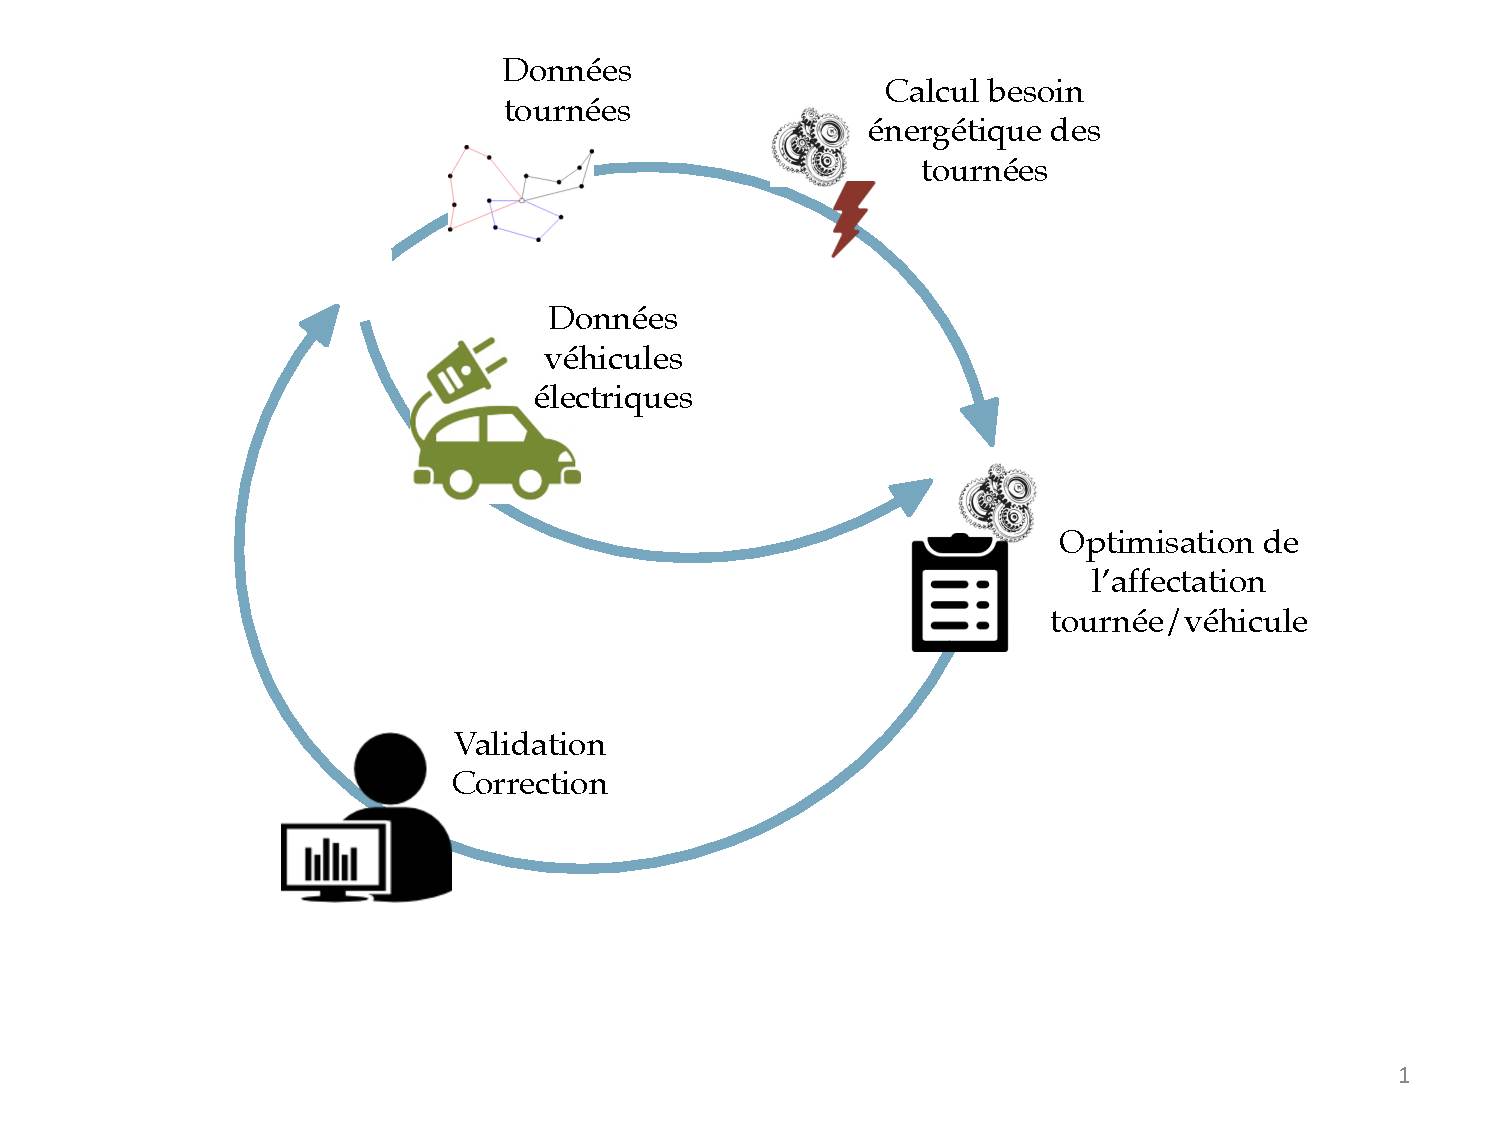
\includegraphics[trim=0cm 3cm 0cm 0cm, width=0.8\textwidth]{figures/5_implementation/processus_metier.pdf}
     \end{center}
     \caption{Processus d'affectation de véhicules électriques à des tournées}
     \label{fig:processus_metier}
    \end{figure}

    Pour ce cas d'étude, l'analyse de la structure exploite les liens de la vue
    intégration et la conformité du modèles d'architecture au métamodèle EA2M.
    L'analyse du comportement consiste à simuler l'ensemble de l'architecture en
    pilotant la simulation par le processus métier. Cette simulation a pour
    objectif de valider et critiquer  les choix de modélisation et d'anticiper
    l'éventuel dimensionnement de la flotte. Par exemple, si une forte
    proportion des tournées implique une distance effectuée supérieure à
    l'autonomie des véhicules électriques sans possibilité de recharge en cours
    de route (pas de borne à disposition au cours de la tournée), la simulation
    permet  de trouver la proportion de véhicules thermiques à garder a minima
    dans une flotte. L'affectation doit aussi privilégier l'utilisation des
    véhicules électriques car la rentabilité d'un parc de véhicules électriques
    est proportionnelle au nombre de kilomètres effectués par ces véhicules.

    \subsection{Mise en œuvre du \emph{framework ExecuteEA}\\
    pour la modélisation des vues métier, fonctionnelle et applicative}

    La première étape consiste donc à créer les modèles des vues métier, fonctionnelle
    et applicative en recourant à des langages de modélisation exécutables. Selon les
    propositions de ces travaux de thèse, l'usage de ces langages automatisent
    la manipulation des modèles et facilitent leur analyse. La
    figure~\ref{fig:architecture_generale_usecase} présente l'architecture \emph{in globo}
    du cas métier ainsi modélisé, selon le cadre structurant \emph{ExecuteEA}.






% Nous éprouvons notre démarche au cas métier de la gestion d'une flotte de
% véhicules électriques. Nous construisons les modèles adéquats pour les vues
% métier, fonctionnelle et applicative en adoptant des langages exécutables. La
% cohérence est modélisée dans la vue intégration. L'architecture globale du cas
% métier est illustrée dans la \ref{fig:architecture_generale_usecase}.


\begin{figure}[!htbp]
 \begin{center}
  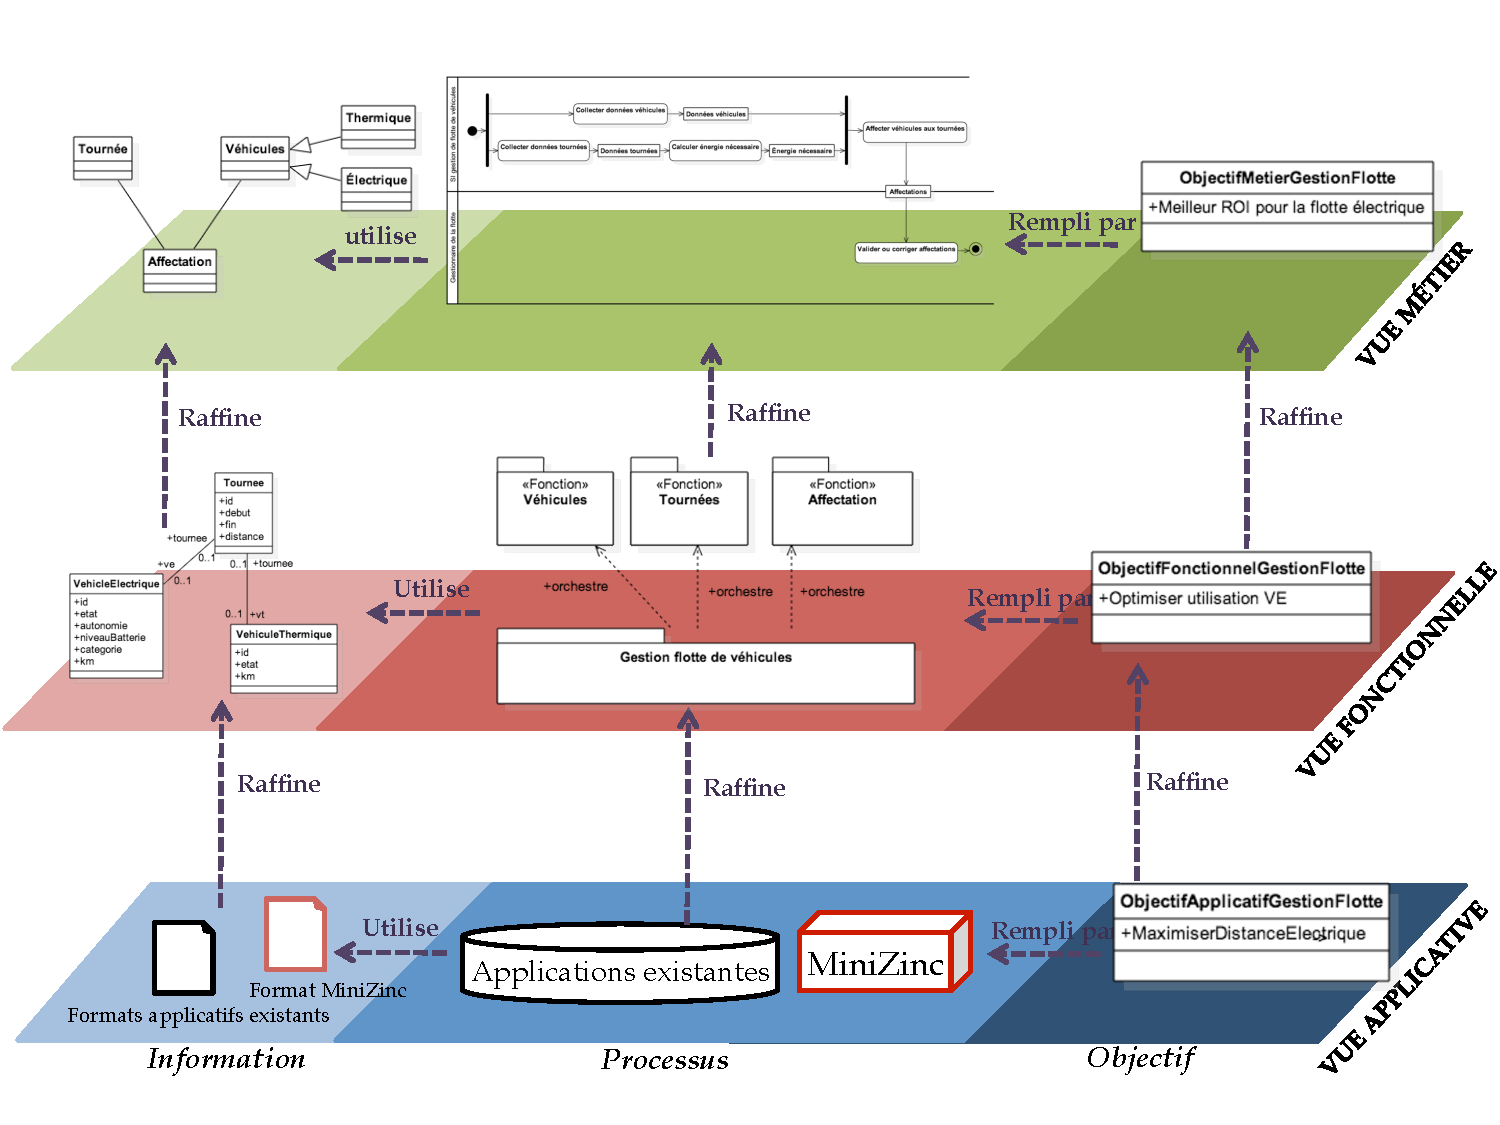
\includegraphics[angle=90, width=1\textwidth]{figures/5_implementation/architecture_generale_usecase.pdf}
 \end{center}
 \caption{Architecture globale du cas d'étude \\mettant en œuvre le \protect\emph{framework ExecuteEA}}
 \label{fig:architecture_generale_usecase}
\end{figure}


\subsubsection{Modélisation de la vue métier} 

Nous utilisons fUML comme langage
exécutable pour modéliser cette vue. Le processus métier consiste à collecter
les données relatives aux véhicules (électriques et thermiques) ainsi qu'aux
tournées à effectuer, de calculer l'énergie nécessaire à chaque tournée et
l'affectation véhicule/tournée avant de faire valider cette dernière par le
manager de flotte. Nous modélisons ce processus métier sous forme de diagramme
d'activité fUML en utilisant l'atelier de modélisation Papyrus. Selon notre cadre
d'architecture, les modèles créés représentent donc l'aspect processus de la vue
métier. La figure~\ref{fig:processus_fuml} présente le diagramme d'activité fUML obtenu à
l'aide de Papyrus.

\begin{figure}[!htbp]
 \begin{center}
  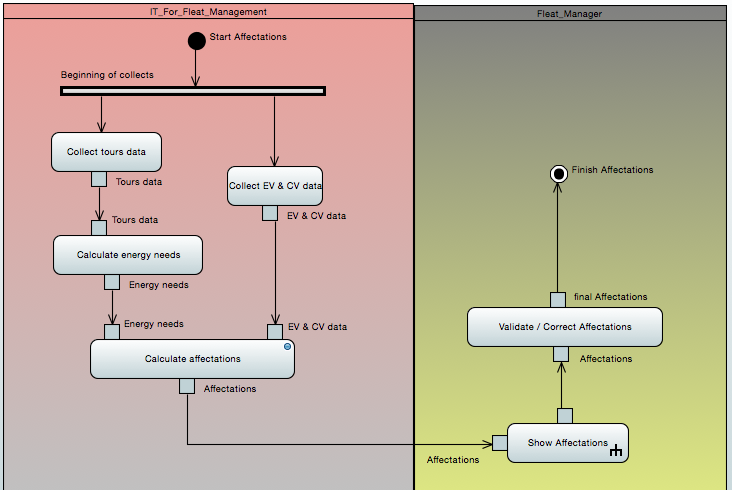
\includegraphics[width=1\textwidth]{figures/5_implementation/processus_fuml.png}
 \end{center}
 \caption{Aspect processus de la vue métier modélisé sous la forme d'un diagramme d'activité fUML avec Papyrus}
 \label{fig:processus_fuml}
\end{figure}


Pour l'aspect information, nous utilisons des diagrammes de classe UML pour
représenter les concepts métier et leurs relations. Nous modélisons ainsi les
concepts de Véhicule, Tournée et Affectation. La figure~\ref{fig:information_metier}
présente le diagramme de classes fUML modélisé dans Papyrus.

\begin{figure}[!htbp]
 \begin{center}
  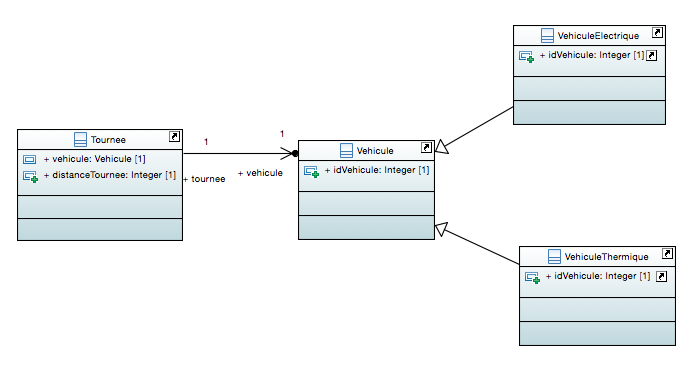
\includegraphics[width=1\textwidth]{figures/5_implementation/information_metier.png}
 \end{center}
 \caption{Aspect information de la vue métier modélisé sous la forme d'un diagramme de classes fUML avec Papyrus}
 \label{fig:information_metier}
\end{figure}

Gérer une flotte de véhicules peut
avoir plusieurs objectifs métier. Dans notre cas, obtenir le meilleur retour sur
investissement suite à l'intégration de véhicules électriques dans la flotte de
véhicules. Nous modélisons l'objectif métier sous la forme d'une classe UML
représentant l'aspect objectif de la vue métier comme l'illustre la 
figure~\ref{fig:architecture_generale_usecase}.

% Le choix des langages de modélisation et de l'outil de simulation est motivé par
% les pratiques du domaine. En effet, la Commission Électrique Internationale a
% adopté Enterprise Architect comme outil pour maintenir et distribuer le
% CIM\footnote{Common Information Model}\cite{uslar2012standardization}, un modèle
% d'information commun pour le domaine électrique
% \footnote{www.sparxsystems.com.au/press/articles/iec.html}.
	

\subsubsection{Modélisation de la vue fonctionnelle}

Nous modélisons l'aspect information de la vue fonctionnelle sous la forme d'un diagramme de classes
fUML. Ce modèle raffine les concepts métier en spécifiant leurs types. Dans la
vue fonctionnelle, le concept d'allocation prend la forme d'une association
entre les véhicules et les tournées. 

\begin{figure}[!htbp]
 \begin{center}
  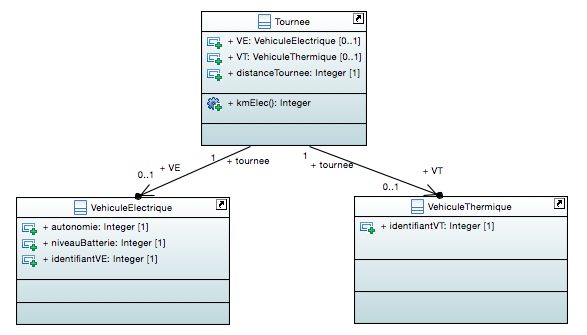
\includegraphics[width=1\textwidth]{figures/5_implementation/information_fonctionnelle.png}
 \end{center}
 \caption{Aspect information de la vue fonctionnelle modélisé sous la forme d'un diagramme de classes fUML avec Papyrus}
 \label{fig:information_fonctionnelle}
\end{figure}

L'objectif fonctionnel est d'optimiser
l'utilisation des véhicules électriques pour atteindre l'objectif métier qui est
d'avoir un meilleur retour sur investissement. Nous modélisons cet objectif 
sous la forme d'une classe UML
représentant l'aspect objectif de la vue fonctionnelle comme l'illustre la 
figure~\ref{fig:architecture_generale_usecase}.

Pour l'aspect processus de la vue fonctionnelle, nous commençons par identifier trois blocs fonctionnels~:
un bloc pour la gestion de la flotte de véhicules (électriques et thermiques),
un bloc pour la gestion des tournées, un bloc pour la gestion de l'affectation
(voir figure \ref{fig:architecture_generale_usecase}. Ces blocs contiennent les
fonctions qui raffinent les tâches du processus métier. Comme expliqué plus tôt
dans la démarche, le fait de les rassembler dans des blocs selon les concepts
métier augmente la modularité et l'évoluvilité de l'architecture. De plus, nous
consacrons un bloc à la gestion des processus fonctionnels. Ce bloc est
responsable de l'orchestration des fonctions du processus fonctionnel.

Les blocs fonctionnels offrent une vue plus détaillée des tâches métier. 
Pour ce cas d'étude, nous détaillons uniquement la tâche métier qui consiste à
affecter un véhicule à une tournée. Nous modélisons l'affectation des véhicules 
aux tournées
sous la forme de contraintes \gls{ocl}~: pour affecter un véhicule à une tournée, il
faut que l'énergie nécessaire à celle-ci soit inférieure à l'autonomie de la
batterie. Dans notre cas d'application, nous considérons qu'il n'est pas
possible de recharge le véhicule pendant la tournée de l'agent.

Nous modélisons la fonction d'affectation sous la
forme de deux contraintes et d'une requête en utilisant OCL. La première contrainte OCL signifie
que si un véhicule électrique est affecté à une tournée alors l'énergie dont il
dispose permet d'assurer la totalité de la tournée. La deuxième contrainte
signifie que si aucun véhicule électrique n'est capable d'assurer une tournée
donnée alors c'est un véhicule thermique qui lui est associé. Enfin, la requête
calcule le nombre total de kilomètres électriques correspondant à la distance
parcourue par les véhicules électrique après l'affectation. Cette requête permet
d'évaluer l'utilisation  des véhicules électriques dans l'optique d'atteindre
l'objectif fonctionnel.

Il est possible de modéliser les autres algorithmes de
traitement (calcul des tournées à partir de bon de travaux, calcul de l'énergie
nécessaire à une tournée, etc.) à l'aide de diagrammes d'activité exécutables.



\lstinputlisting[caption=Contraintes OCL pour la fonction d'affectation]{figures/5_implementation/tournee.ocl}

\subsubsection{Modélisation de la vue applicative}

Pour les processus applicatifs, nous commençons par identifier  les applications
nécessaires à l'implantation des blocs fonctionnels. Dans notre cas, le
patrimoine applicatif de l'entreprise dispose déjà d'applications pour la
gestion de tournées (calcul de tournées optimisé à partir de bons de travaux) et
la gestion de véhicules (administration, maintenance, etc.). Pour la fonction
d'allocation, nous faisons le choix d'utiliser MiniZinc pour modéliser les
contraintes au niveau applicatif \ref{fig:contraintesMiniZinc}.

\begin{figure}[!htbp]
 \begin{center}
  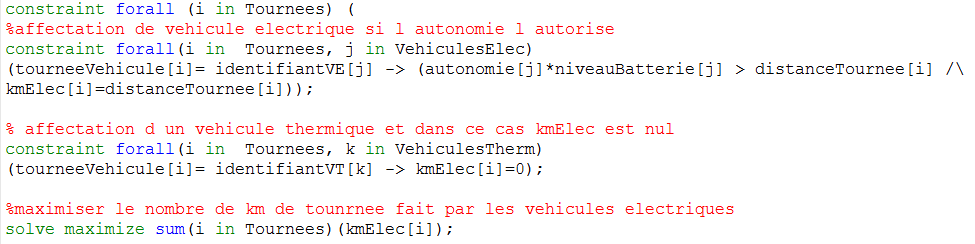
\includegraphics[width=1\textwidth]{figures/5_implementation/module_minizinc.png}
 \end{center}
 \caption{Contraintes du module MiniZinc}
 \label{fig:contraintesMiniZinc}
\end{figure} 

MiniZinc est un langage de modélisation et de résolution de contraintes de
niveau intermédiaire qui a pour vocation de devenir un langage de modélisation
standard dans le domaine de la programmation par contraintes. L'aspect
information contient les formats de données nécessaires aux différentes
applications. La figure \ref{fig:formatMiniZinc} représente le fichier de
données (le format .dzn) nécessaire à l'application MiniZinc pour calculer
l'affectation.

\begin{figure}[!htbp]
 \begin{center}
  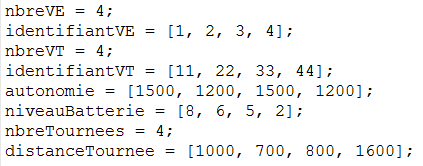
\includegraphics[width=0.5\textwidth]{figures/5_implementation/format_minizinc.png}
 \end{center}
 \caption{Fichier de données pour le module MiniZinc}
 \label{fig:formatMiniZinc}
\end{figure} 

Nous modélisons l'objectif applicatif sous la forme d'une classe UML
représentant l'aspect objectif de la vue applicative comme l'illustre la
figure~\ref{fig:architecture_generale_usecase}. Un véhicule électrique devient
rentable par rapport à un véhicule thermique à partir d'un certain nombre de
kilomètre parcouru. C'est pourquoi l'objectif fonctionnel qui est d'optimiser
l'usage de la flotte électrique se traduit par la maximisation du nombre de
kilomètres électriques, c'est à dire affecter aussi souvent que possible un
véhicule électrique aux tournées. Ainsi, le module MiniZinc prend en compte cet
objectif en résolvant les contraintes tout en maximisant la distance électrique.



\subsection{Intégration et analyse de la structure}

L'approche conceptuelle que nous proposons pour le \emph{framework ExecuteEA},
illustrée par la figure~\ref{fig:approche_conceptuelle} à la
page~\pageref{fig:approche_conceptuelle}, met l'accent sur le rôle intégrateur
de l'architecte d'entreprise~: il doit s'assurer de la cohérence intra-vue et
inter-vues de l'architecture globale tout en collaborant avec les architectes
métier, fonctionnel et applicatif.

L'intégration de l'architecture passe par la modélisation de la vue intégration,
c'est-à-dire par la spécification des liens de cohérence  intra-vue et et inter-
vues conformément au métamodèle EA2M. Nous avons donc modélisé ces liens pour
l'ensemble des vues métier, fonctionnelle et applicative. Néanmoins, la figure
\ref{fig:integration_gestion_flotte} ne présente qu'une partie modèles
d'intégration pour des raisons de lisibilité. Nous y modélisons à titre
d'illustration les liens de cohérence intra-vue entre la fonction d'affection,
ses inputs et output en termes de types fonctionnels, ainsi que son objectif
fonctionnel. Nous faisons de même pour le module d'optimisation MiniZinc, ses
inputs et outputs ainsi que l'objectif applicatif qu'il remplit. Le même
principe d'intégration intra-vue, c'est à dire entre les aspects d'une même vue,
est applicable à tous les autres éléments de la vue métier, fonctionnelle et
applicative.

\begin{figure}[!htbp]
 \begin{center}
  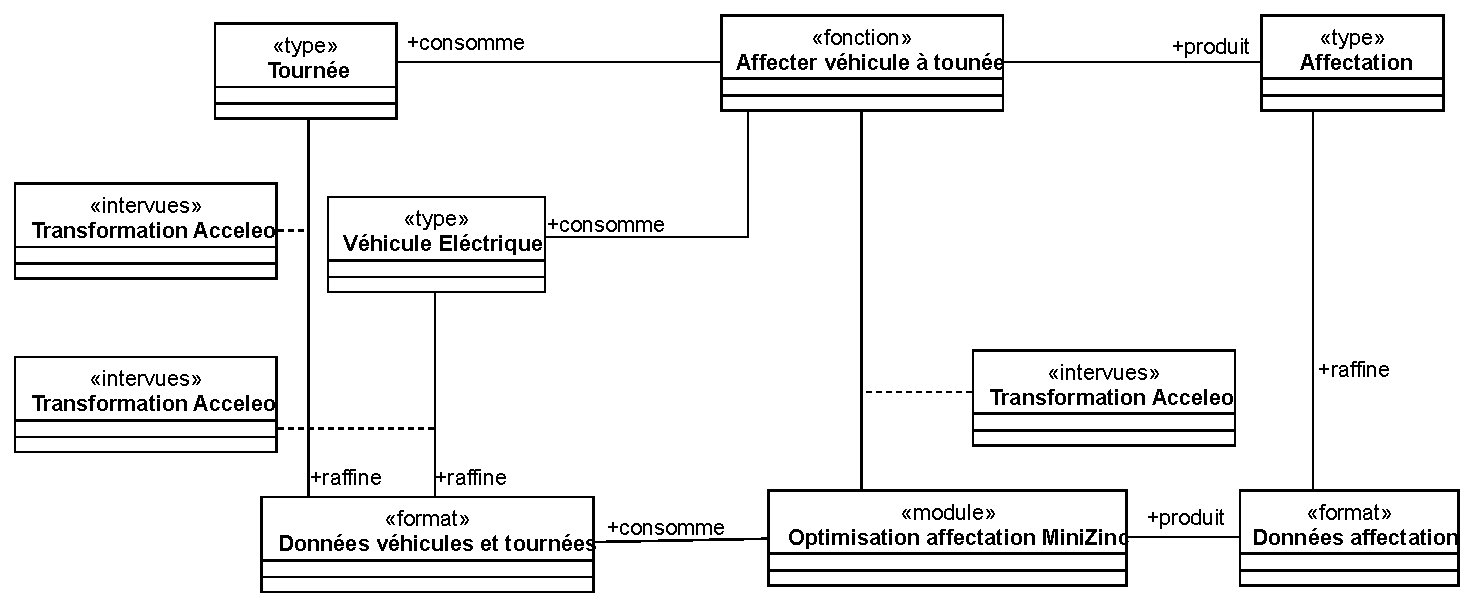
\includegraphics[trim= 0cm 0cm 0cm 0cm, width=1\textwidth]{figures/5_implementation/integration_affectation.pdf}
 \end{center}
 \caption{Une vue partielle des modèles d'intégration \\de la vue fonctionnelle et de la vue applicative}
 \label{fig:integration_gestion_flotte}
\end{figure}

De la même manière, nous modélisons les liens de cohérence inter-vues. Par
exemple, le lien \q{consomme} exprime qu'un type de données est compatible avec
la fonction qui l'utilise et qu'un format est compatible avec le module
applicatif qui l'utilise en entrée. Pour garantir une bonne orchestration des
processus, il faut que le \q{produit} d'une tâche (respectivement une fonction,
un module applicatif) soit compatible avec le ce que produit la tâche suivante
(respectivement une fonction, un module applicatif).

L'intégration passe aussi par l'identification des éventuelles transformation de
modèles. Rappelons ici que les transformations ont pour objectif d'améliorer
l'alignement métier/IT en automatisant le passage d'une vue à une autre. Pour le
cas métier de la gestion de flotte de véhicules, nous utilisons une
transformation de modèle pour générer les contraintes pour le module de calcul
d'affectation MiniZinc de la vue applicative à partir des contraintes OCL
exprimées dans la fonction affectation de la vue fonctionnelle. La
transformation est écrite dans le langage de transformation Acceleo. En plus de
transformer les contraintes décrite dans l'aspect métier, cette transformation
de modèle permet aussi de transformer les instances des types fonctionnels en
instances dans le format \q{.dzn} utilisé par le module MiniZinc comme
l'illustre la figure \ref{fig:integration_gestion_flotte}. La génération de code
pour le module MiniZinc peut être lancée à partir de la vue fonctionnelle que
nous avons précédemment modélisée dans Papyrus comme l'illustre la
figure~\ref{fig:acceleo_papyrus}.

\begin{figure}[!htbp]
 \begin{center}
  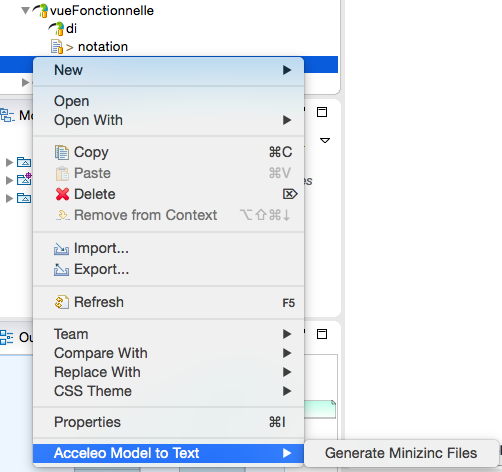
\includegraphics[width=0.7\textwidth]{figures/5_implementation/acceleo_papyrus.png}
 \end{center}
 \caption{Génération du code pour le module MiniZinc\\à partir de la vue fonctionnelle dans Papyrus}
 \label{fig:acceleo_papyrus}
\end{figure}


\subsection{Simulation et analyse du comportement}

Grâce aux langages exécutables, l'analyse du comportement des modèles
d'architecture se fait directement dans les langages de modélisation utilisés
pour les vues. Avec le \emph{framework} ExecuteEA, nous proposons de simuler de
l'ensemble de l'architecture en la pilotant par l'exécution du processus métier.
La simulation du processus métier se traduit par l'exécution du diagramme
d'activité fUML à l'aide du moteur d'exécution Moka intégré à Papyrus. Un des
avantages de l'outil Papyrus est de permettre la modélisation \emph{et} la
simulation de l'architecture dans un même environnement.

Notre approche préconise de modéliser les détails des taches dans les vues
inférieure afin de respecter le niveau d'abstraction requis par chaque point de
vue et ainsi de ne pas altérer la compréhension des parties prenantes de la vue
qui leur destinée. Par exemple, l'analyse métier n'aura ainsi pas à discuter du
détails des applications implémentant les tâches métier avec l'architecte
applicatif.

Comme expliqué dans la section~\ref{sec:opaque_action_papyrus}, Papyrus offre la
possibilité d'étendre la sémantique d'exécution de fUML à travers les
\emph{Opaque Action}. Celles-ci permettent d'invoquer des modules d'applications
extérieures au moment de l'exécution du diagramme d'activité fUML.
Développée pour les besoins du cas d'étude, cette extension rend possible l'invocation directe
du module MiniZinc pendant l’exécution du processus métier pour optimiser
l'affectation des véhicules aux tournées. Rappelons que le module MiniZinc est
obtenu par transformation de modèle à partir de la vue fonctionnelle.

La simulation prend la forme d'une animation de diagramme. La figure
\ref{fig:simu_capture_ecran} est une capture d'écran montrant la simulation du processus métier
en cours d'exécution. Papyrus offre la possibilité de mettre des \emph{breakpoints} sur
certaines activités et de paramétrer le pas de temps pour contrôler le
déroulement du processus.

\begin{figure}[!htbp]
 \begin{center}
  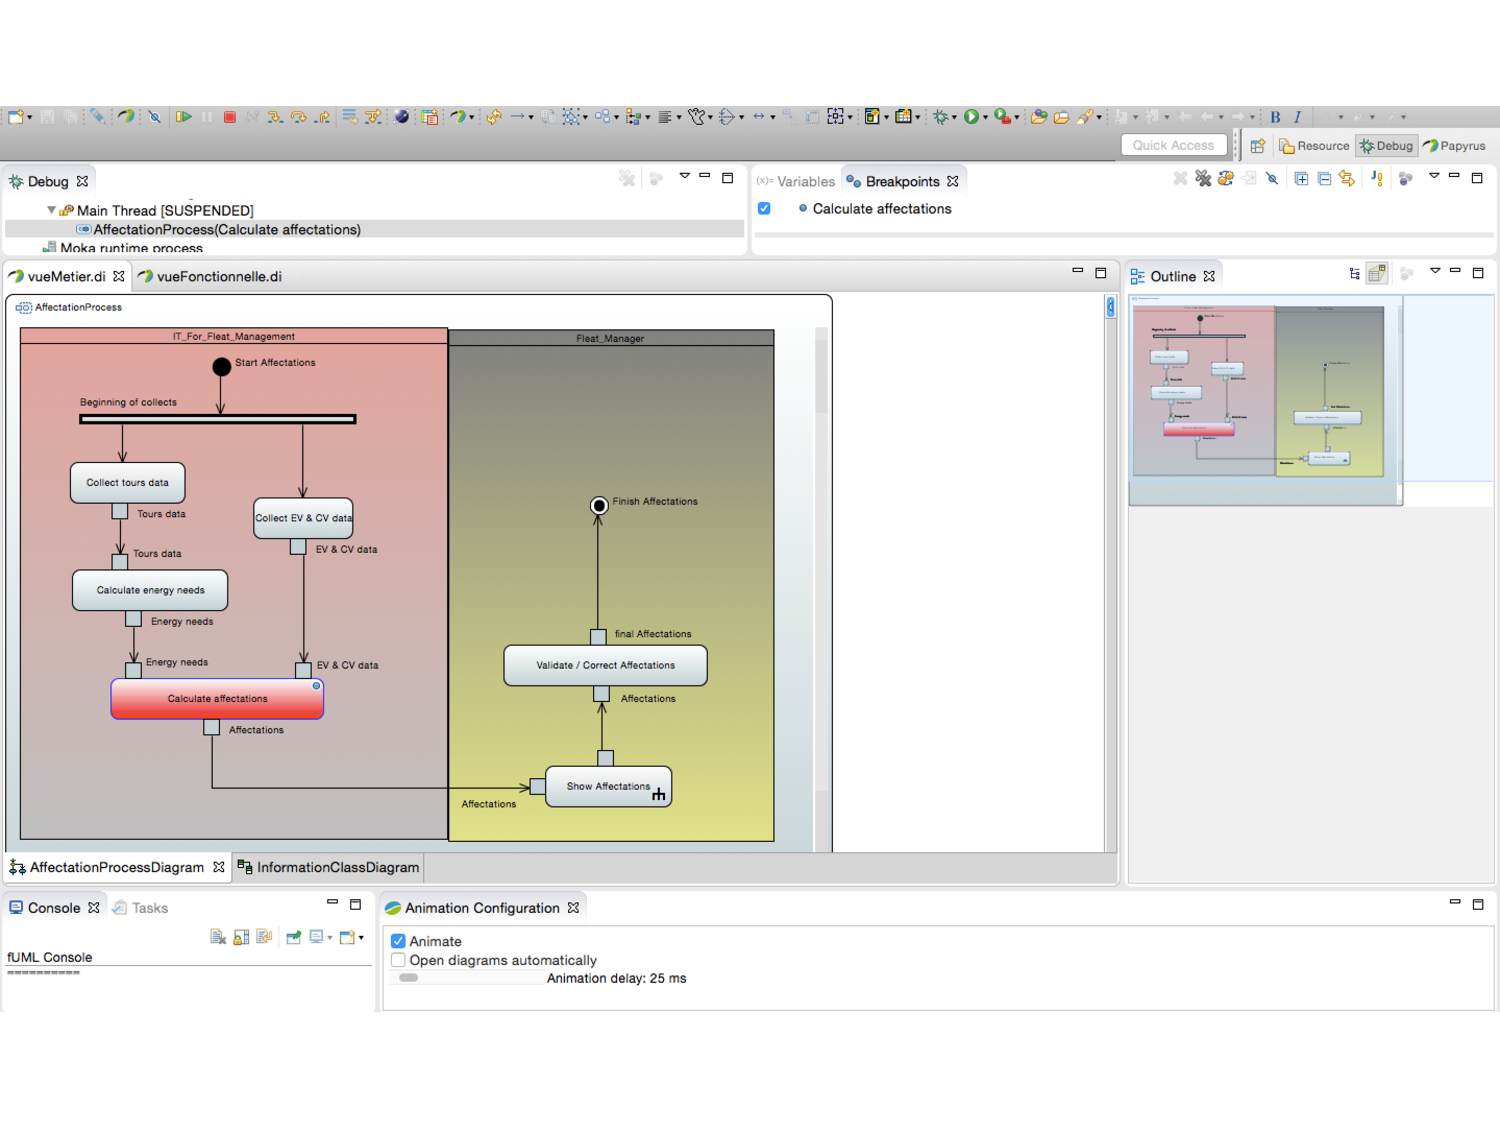
\includegraphics[angle=90, width=1\textwidth]{figures/5_implementation/simu_capture_ecran.pdf}
 \end{center}
 \caption{Simulation de l'architecture sous Papyrus}
 \label{fig:simu_capture_ecran}
\end{figure}

La simulation retourne comme résultat les affectations des véhicules aux
tournées. Ce résultat est affiché dans la console fUML comme l'illustre la
figure \ref{fig:resultat_simu}. La simulation a pour objectif de voir si
l'utilisation des véhicules électrique est rentable en comparant la distance
parcourue par le véhicule électrique et la distance minimale permettant de le
rentabiliser. Dans ce cas, il est par exemple envisageable de reconfigurer les
tournées de manière à ce que plus de véhicules électriques soient affectés. En
effet, notre démarche a pour but l'analyse fonctionnelle. La validation s'appuie
sur les indicateurs dérivés de l'aspect objectif et sur l'avis des experts. Des
analyses statistiques peuvent être conduites mais elles ne rentrent pas dans le
périmètre de nos travaux.

\begin{figure}[!htbp]
 \begin{center}
  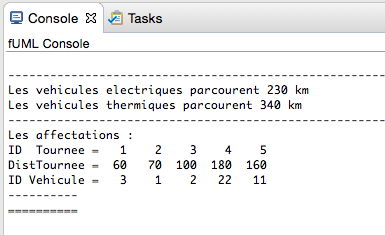
\includegraphics[width=0.6\textwidth]{figures/5_implementation/resultat_simu.png}
 \end{center}
 \caption{Résultat retourné par la simulation du cas d'étude dans Papyrus}
 \label{fig:resultat_simu}
\end{figure} 

Comme exposé dans l'état de l'art, l'approche ExecuteEA s'inscrit dans l'école
de pensée \emph{Enterprise System Architecting}~: par l'analyse du comportement
de l'architecture, nous souhaitons non seulement vérifier l'alignement de l'IT à
la stratégie de l'entreprise mais aussi donner la possibilité au métier
d'évaluer sa propre stratégie en fonction de sa déclinaison au niveau de l'IT.
Dans le contexte de la gestion d'une flotte de véhicules électriques, la
simulation peut aboutir à la non adéquation du type de tournées avec l'impératif
de rentabiliser l'investissement dans une flotte de véhicules électriques à
cause de la distance des tournées. En pareil cas, les architectes —~métier,
fonctionnel et applicatif~— en étroite collaboration avec l'architecte
d'entreprise peuvent envisager de faire évoluer l'application qui optimise les tournées quotidiennes 
crées à partir des bons de travaux pour en écourter la distance.




%\section{analyse de la structure}
%Validate modèle -> pour tester l'intégrité du modèle
%Requêtes sur le modèle OCL
%Si appli hirs service quel sont les processus impacté etc.
%Un nouveau process faisant intervenir d'ancienne tâche, quelle ancienne appli réutilisée
%Détecter les problèmes d'interop' entre modules
 
%\lstinputlisting{figures/5_implementation/affectations.mzn}

\section[Discussion et perspectives]{Discussion et perspectives pour le prototypage\\
            et la validation du \emph{framework} ExecuteEA}

    Le développement du prototype et son application au cas métier
    de la gestion d'une flotte de véhicules électriques concrétise l'ensemble des
    propositions autour du \emph{framework} ExecuteEA et du métamodèle EA2M
    et fournit un outil d'analyse de la structure et du comportement
    d'une architecture d'entreprise.

    Bien que nous n'avons modélisé et simulé qu'un seul processus métier, la mise
    en œuvre du \emph{framework} ExecuteEA a permis de valider les apports de l'IDM
    en tant que cadre technologique et méthodologique aux différentes activités d'EA.
    La première limite de cet implémentation est donc le passage à l'échelle. C'est en effet dans le
    traitement d'une grande quantité d'artefacts utiles à l'EA, dont la gestion dépend souvent du 
    savoir-faire de l'architecte d'entreprise uniquement
    sans assistance informatique particulière, que notre  proche prouve sa valeur.

    Une premier passage à l'échelle serait donc de d'élargir le cas métier en incluant par exemple
    le processus de calcul de tournées journalières à partir de bons de travaux, le processus
    de recharge de la batterie et ses impacts sur le réseau électrique, le processus d'entretien des
    voitures, le processus de réservation de voitures par d'autres agents non impliqués dans les tournées,
    etc. 

    Lors de la simulation du processus métier, nous avons implémenté la
    tâche de l'affectation de véhicules aux tournées. Cette implémentation a consisté à modéliser
    la fonction qui réalise cette tâche sous la forme de contraintes OCL puis à obtenir par transformation
    de modèle le code pour le module MiniZinc de la vue applicative. 
    Ces développements valident le principe
    de simulation que nous proposons (cf. figure~\ref{fig:Simulation_Approche} page~\pageref{fig:Simulation_Approche}).
    Il serait donc intéressant de l'étende au reste des tâches métier du processus en utilisant cette fois des diagrammes
    d'activité fUML pour modéliser et simuler leur comportement.

    De manière générale, bien qu'il ne s'agisse que d'un prototype, l'implémentation de la vue intégration avec EMF
    a permis de mettre en lumière les avantages que présente la méta-modélisation pour l'analyse structurelle
    des modèles d'architecture, notamment grâce à la relation de conformité qui lie un modèle à son métamodèle.
    La méta-modélisation avec Ecore est d'autant plus pertinente avec le recours aux contraintes OCLinEcore
    permettant de préciser d'avantage le métamodèle EA2M. Ces mêmes contraintes peuvent aussi servir à
    exprimer des requêtes sur le modèles. À titre d'exemple, nous sommes en train de développer des requêtes
    permettant de retrouver toutes les tâches (respectivement
    fonctions et modules) utilisant un certain concept (respectivement type et format). Une multitude de requêtes de ce
    type gagnent à être développées pour faciliter l'analyse structurelle de l'architecture.

    Enfin, la question de l'adoption des langages de modélisation par les différents parties-prenantes (architectes
    d'entreprise, métier, fonctionnel, applicatif) est cruciale. Bien que l'utilisation de UML comme
    langage de modélisation n'est pas évident de prime abord par des personnes à profile non technique,
    les spécifications des use case Smart Grids recourent de plus en plus à UML au sein de la \gls{cei}.
    Les entretiens menés avec les différents experts d'EA et du réseau électrique révèlent cependant la frilosité
    de certaines personne à adopter UML pour décrire leurs spécifications dans leur intégralité. Néanmoins, ces
    personnes recourent de plus en plus à certains diagrammes comme les diagrammes d'activités pour décrire
    leurs processus. Dans ce contexte, le choix de fUML et de OCL nous semble être \q{raisonnable}.  

    % De manière nous avons mis l'accent sur la simulation est pas assez sur l'analyse de la structure. 

